%% TIPO DE DOCUMENTO 

\documentclass{beamer}

\usetheme{Madrid}
\usecolortheme{seagull}
\usefonttheme{professionalfonts}

%%% IMPORTAMOS PAQUETES A USAR 

\usepackage[utf8]{inputenc}
%\usepackage[latin1]{inputenc}
\usepackage[spanish, es-tabla]{babel}
\usepackage{csquotes}
\usepackage{float}
\usepackage{graphicx}
\usepackage{hyperref}
%Pruebas para animaciones
\usepackage{animate}
\usepackage[document]{ragged2e}
\usepackage{bibentry}
\usepackage{graphicx} % Allows including images
\usepackage{booktabs} % Allows the use of \toprule, 
\usepackage{pgfpages}
%%%START APA
%\usepackage[british]{babel}
%\usepackage[backend=biber,style=apa]{biblatex} OJO CON ESTA LINEA
\setbeamertemplate{navigation symbols}{} % To remove the navigation symbols from the bottom of all slides uncomment this line
%\DeclareLanguageMapping{british}{british-apa}
%\addbibresource{references.bib}

%\setbeameroption{show notes on second screen=left}

%% APA citing
%% \cite{t} - Uthor und Richter, 2010
%% \textcite{t} - Uthor und Riter (2010)
%% \parencite{t} - (Uthor & Riter, 2010)
%% \parencite[Chapt.~4]{t} - (Uthor & Riter, 2010, S. 15)
%%%END APA

%%%%% =================  PORTADA ================== 

\title[Bienvenida] 
{Astronomía para NO astrónomos \\ Los inicios de la Astronomía}
%\subtitle {ne compléter que si l'article possède un sous-titre}

\author[Victor M. Santos] 
%\author[Pedro A. Salgado-Meza ]
{Victor M. Santos \inst{} \and M.Tarazona-Alvarado \inst{}} %\inst{1} \inst{3}}
%{P. A. ~Salgado-Meza\inst{1} \inst{2}}%\and I.~Borne\inst{1} \and J.~Buisson\inst{2}}

\institute[]{
\inst{}Grupo Halley, Escuela de Física, Universidad Industrial de Santander, Bucaramanga, Colombia.}
%\institute[]
%{
%  \inst{1}%
%  Universidad Industrial de Santander, Bucaramanga, Colombia
%  \and
%  \inst{2}%
%  Escuela de Ingenierías Eléctrica, Electrónica y Telecomunicaciones
%  \and
%  \inst{3}%
%  Escuela de Ingeniería Mecánica  
%  }

\date{\today}


\begin{document}
\logo{\includegraphics[scale=2]{Imagenes/Logo_Halley}} 

%%%%%%%%%%%%%%%%%%%%%%%%%%%%%%%%%%%%%%%%%%%%%%%%%%%%%%%%%%%%%%%%%%%%%%
\begin{frame}
\titlepage % Print the title page as the first slide
\end{frame}

%%%%%%%%%%%%%%%%%%%%%%%%%%%%%%%%%%%%%%%%%%%%%%%%%%%%%%%%%%%%%%%%%%%%%%

\begin{frame}{Observando el cielo}
 \begin{columns}
 \column{.45\textwidth}
 ¿Es posible observar el cielo sin telescopios?
  \begin{figure}
 \centering
%\raggedright
 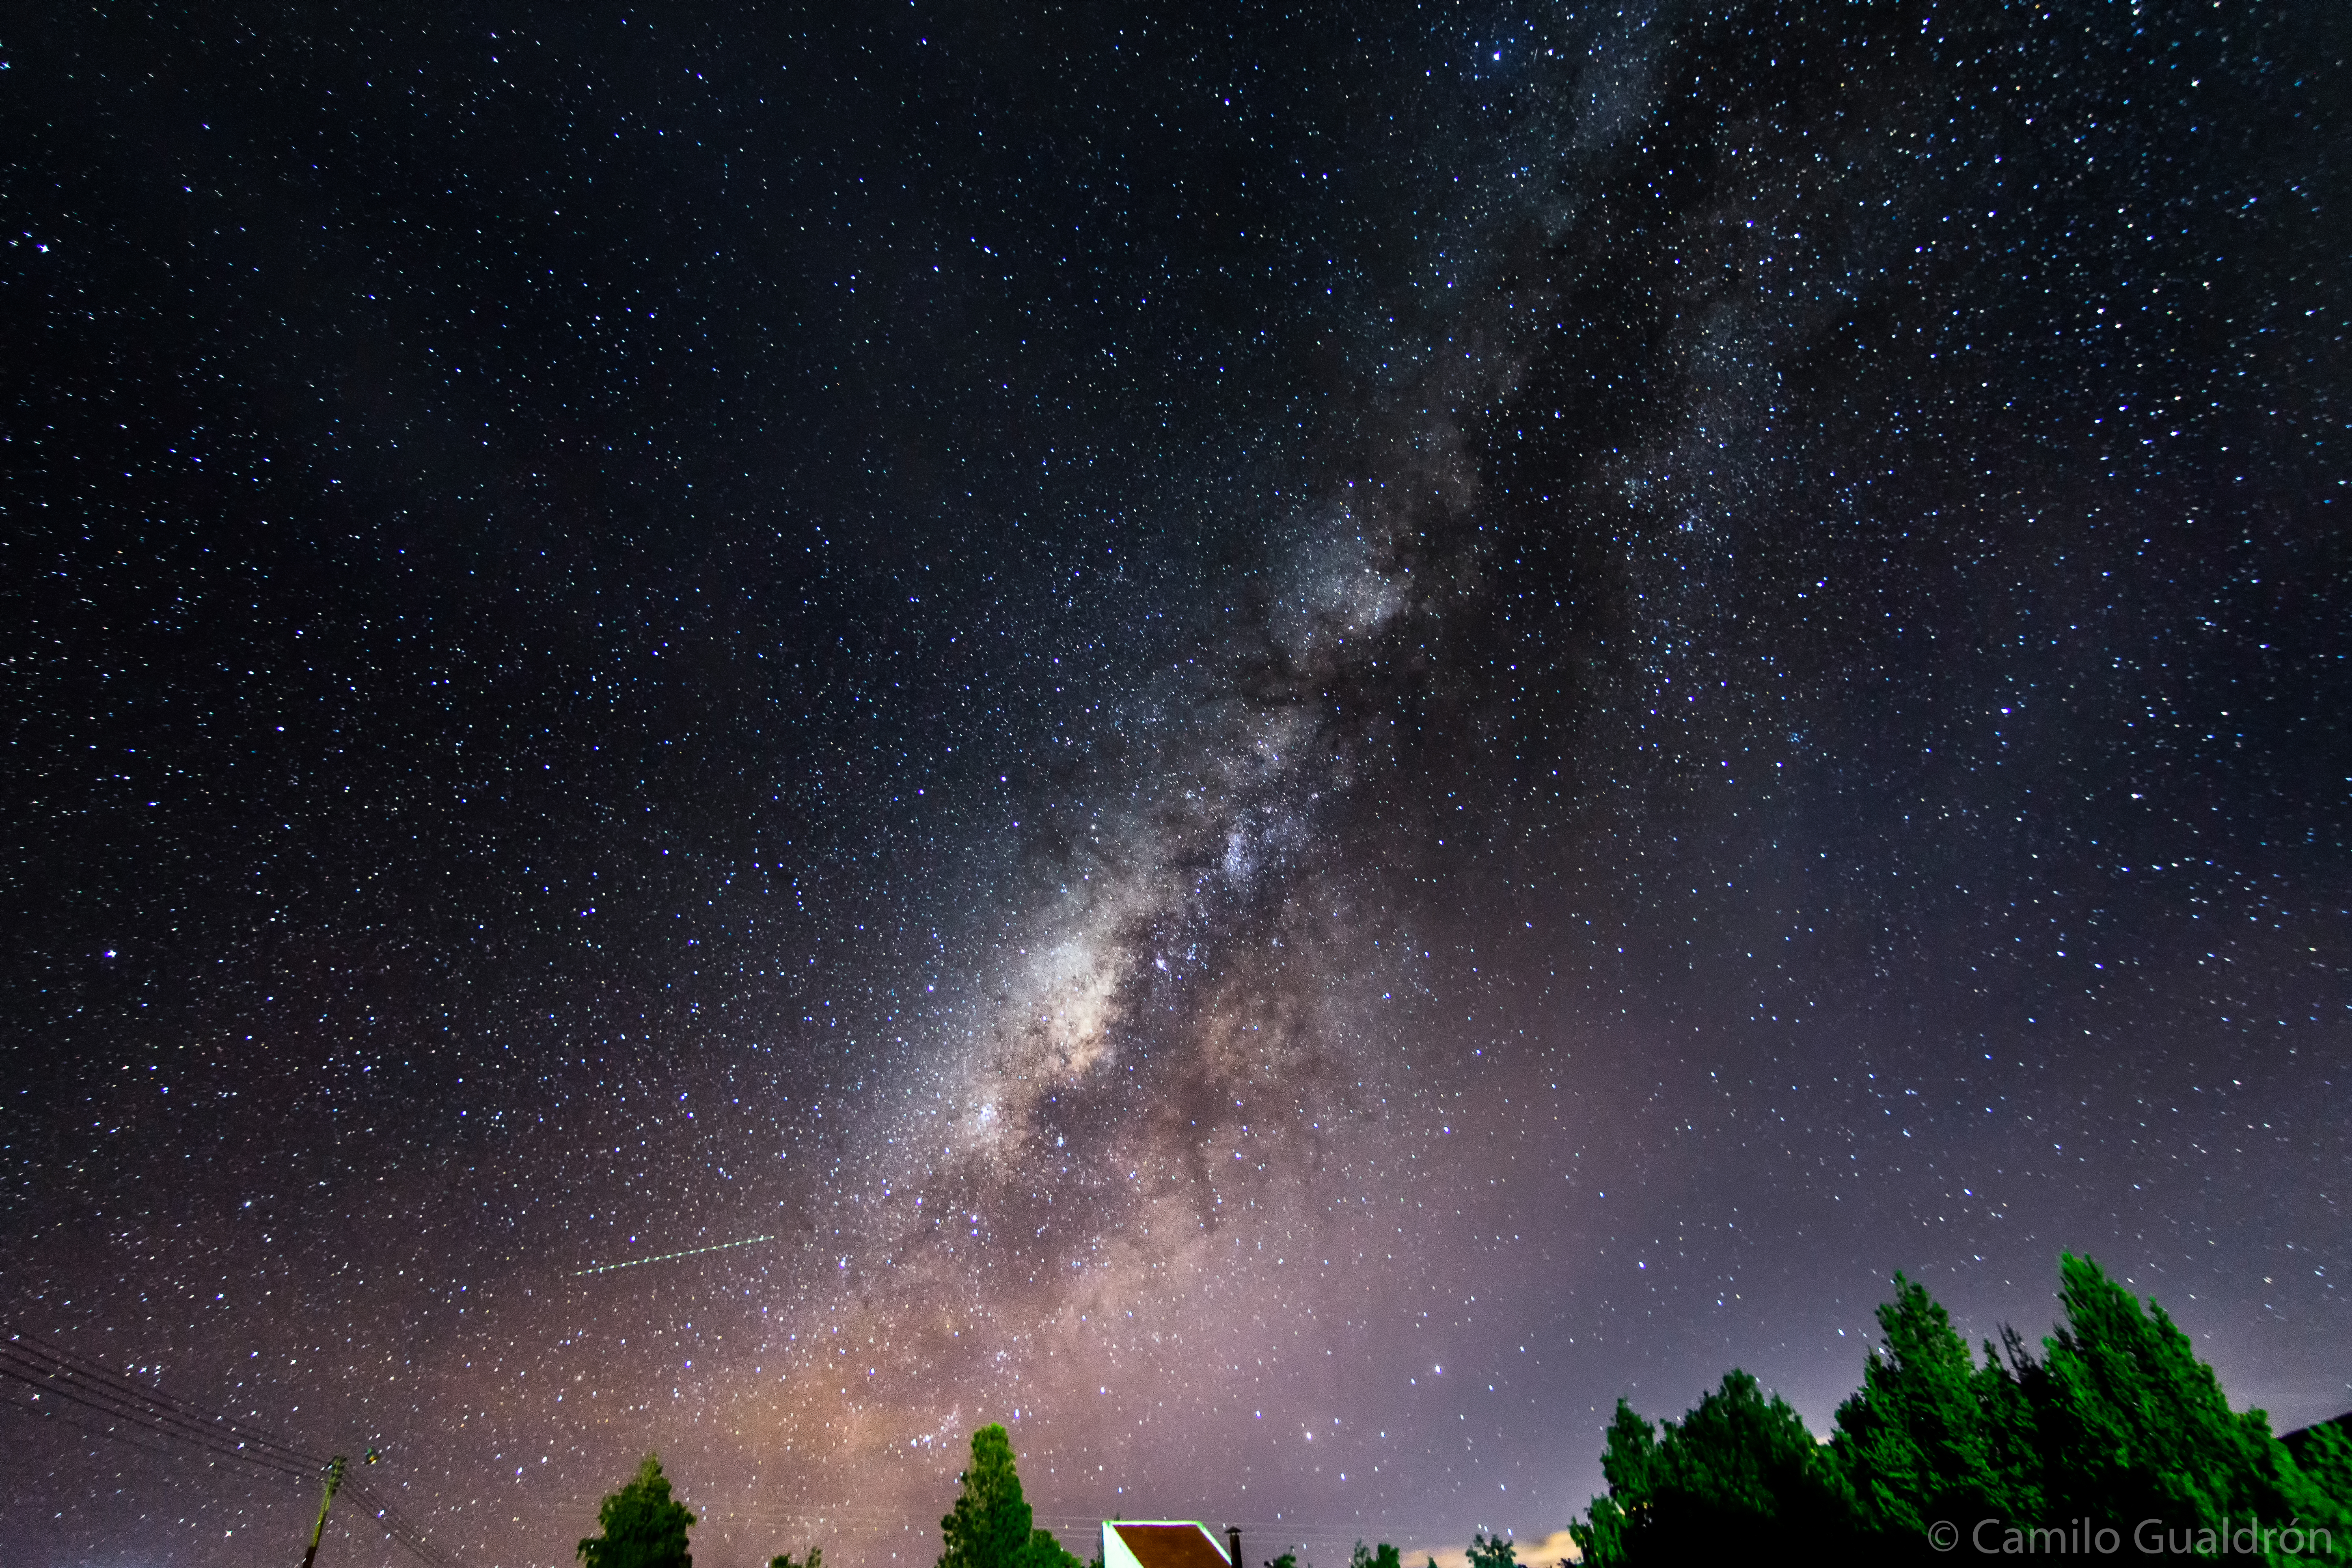
\includegraphics[scale=0.2]{Imagenes/cielo_estrellado_1}
 \end{figure}
 \begin{center}
 \small
 Fotografía: Camilo Gualdron 
 \end{center}
 \column{.45\textwidth}
 ¿Qué necesitamos para observar los astros?\\
 
 \begin{figure}
 \centering
%\raggedright
 \includegraphics[scale=0.022]{Imagenes/cielo_estrellado_2}
 \end{figure}
 \begin{center}
 \small
 Fotografía: Pedro Salgado 
 \end{center}
 \end{columns}
 
 \note{aaaaaaa}
\end{frame}

%%%%%%%%%%%%%%%%%%%%%%%%%%%%%%%%%%%%%%%%%%%%%%%%%%%%%%%%%%%%%%%%%%%%%%%%%%%%%%%%%%%

\begin{frame}
\begin{figure}
 \centering
%\raggedright
 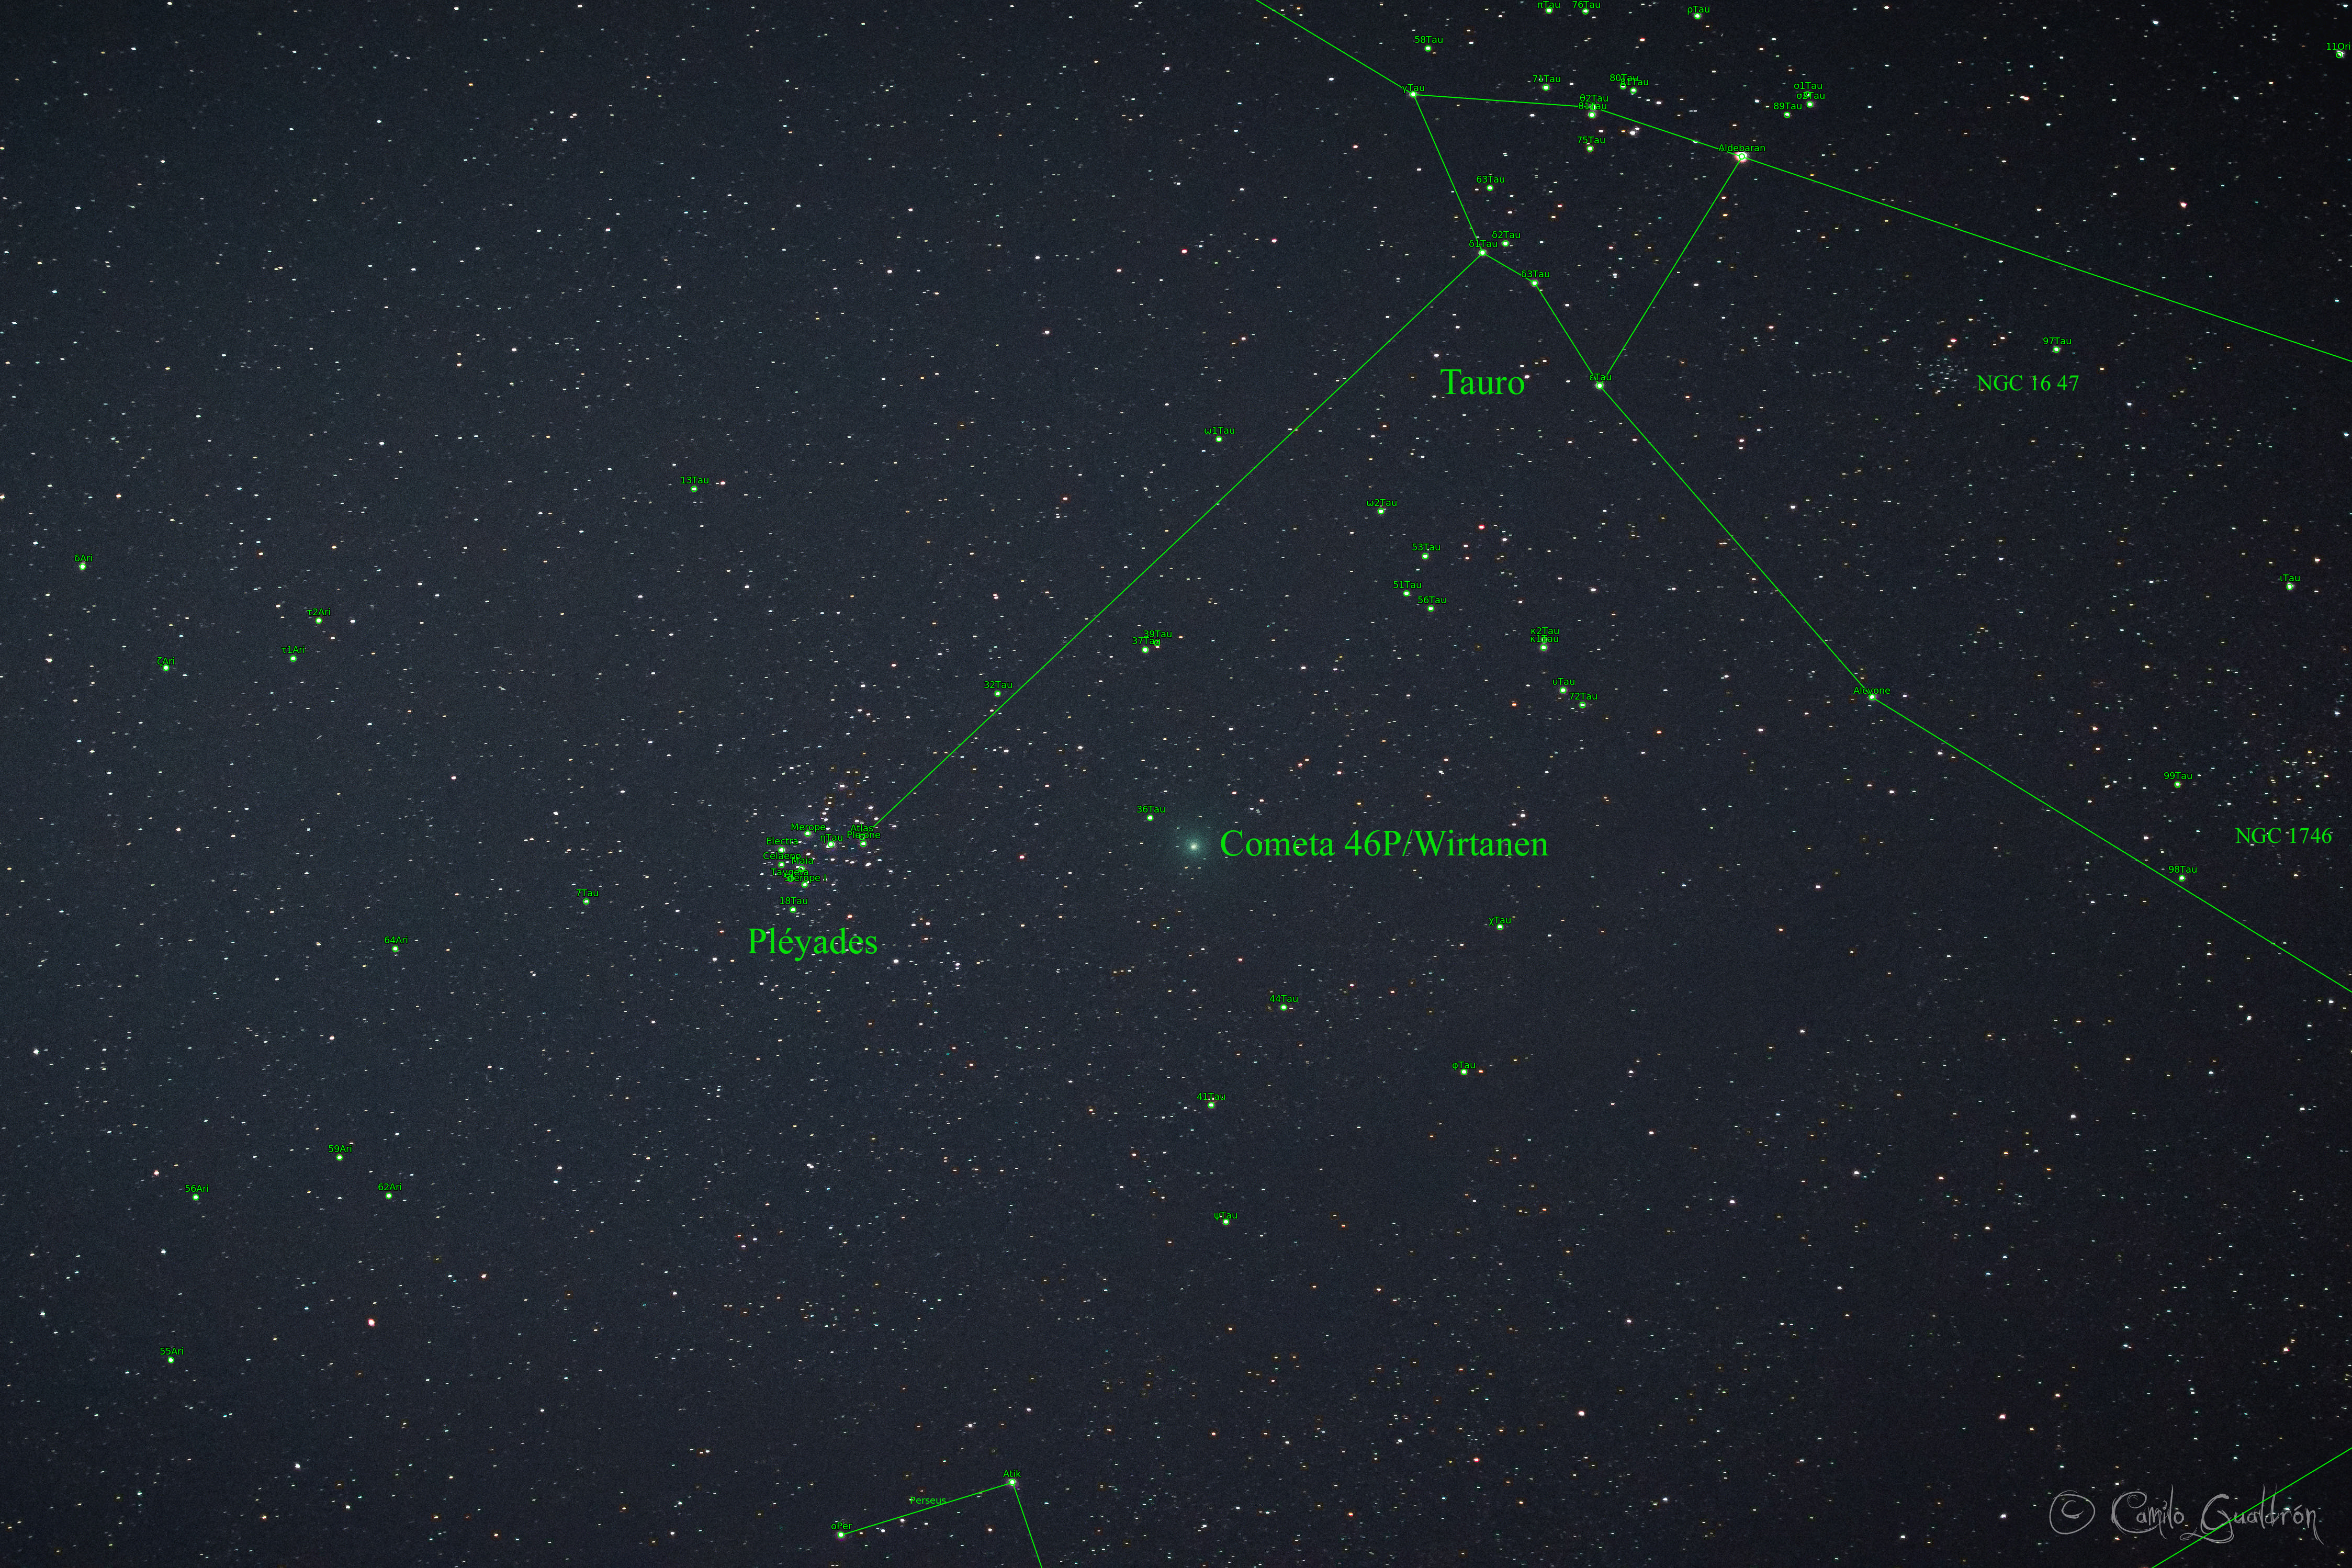
\includegraphics[scale=0.07]{Imagenes/Constelaciones}
 \end{figure}
\end{frame}

%%%%%%%%%%%%%%%%%%%%%%%%%%%%%%%%%%%%%%%%%%%%%%%%%%%%%%%%%%%%%%%%%%%%%%%%%%%%%%%%%%%

\begin{frame}
\begin{figure}
 \centering
%\raggedright
 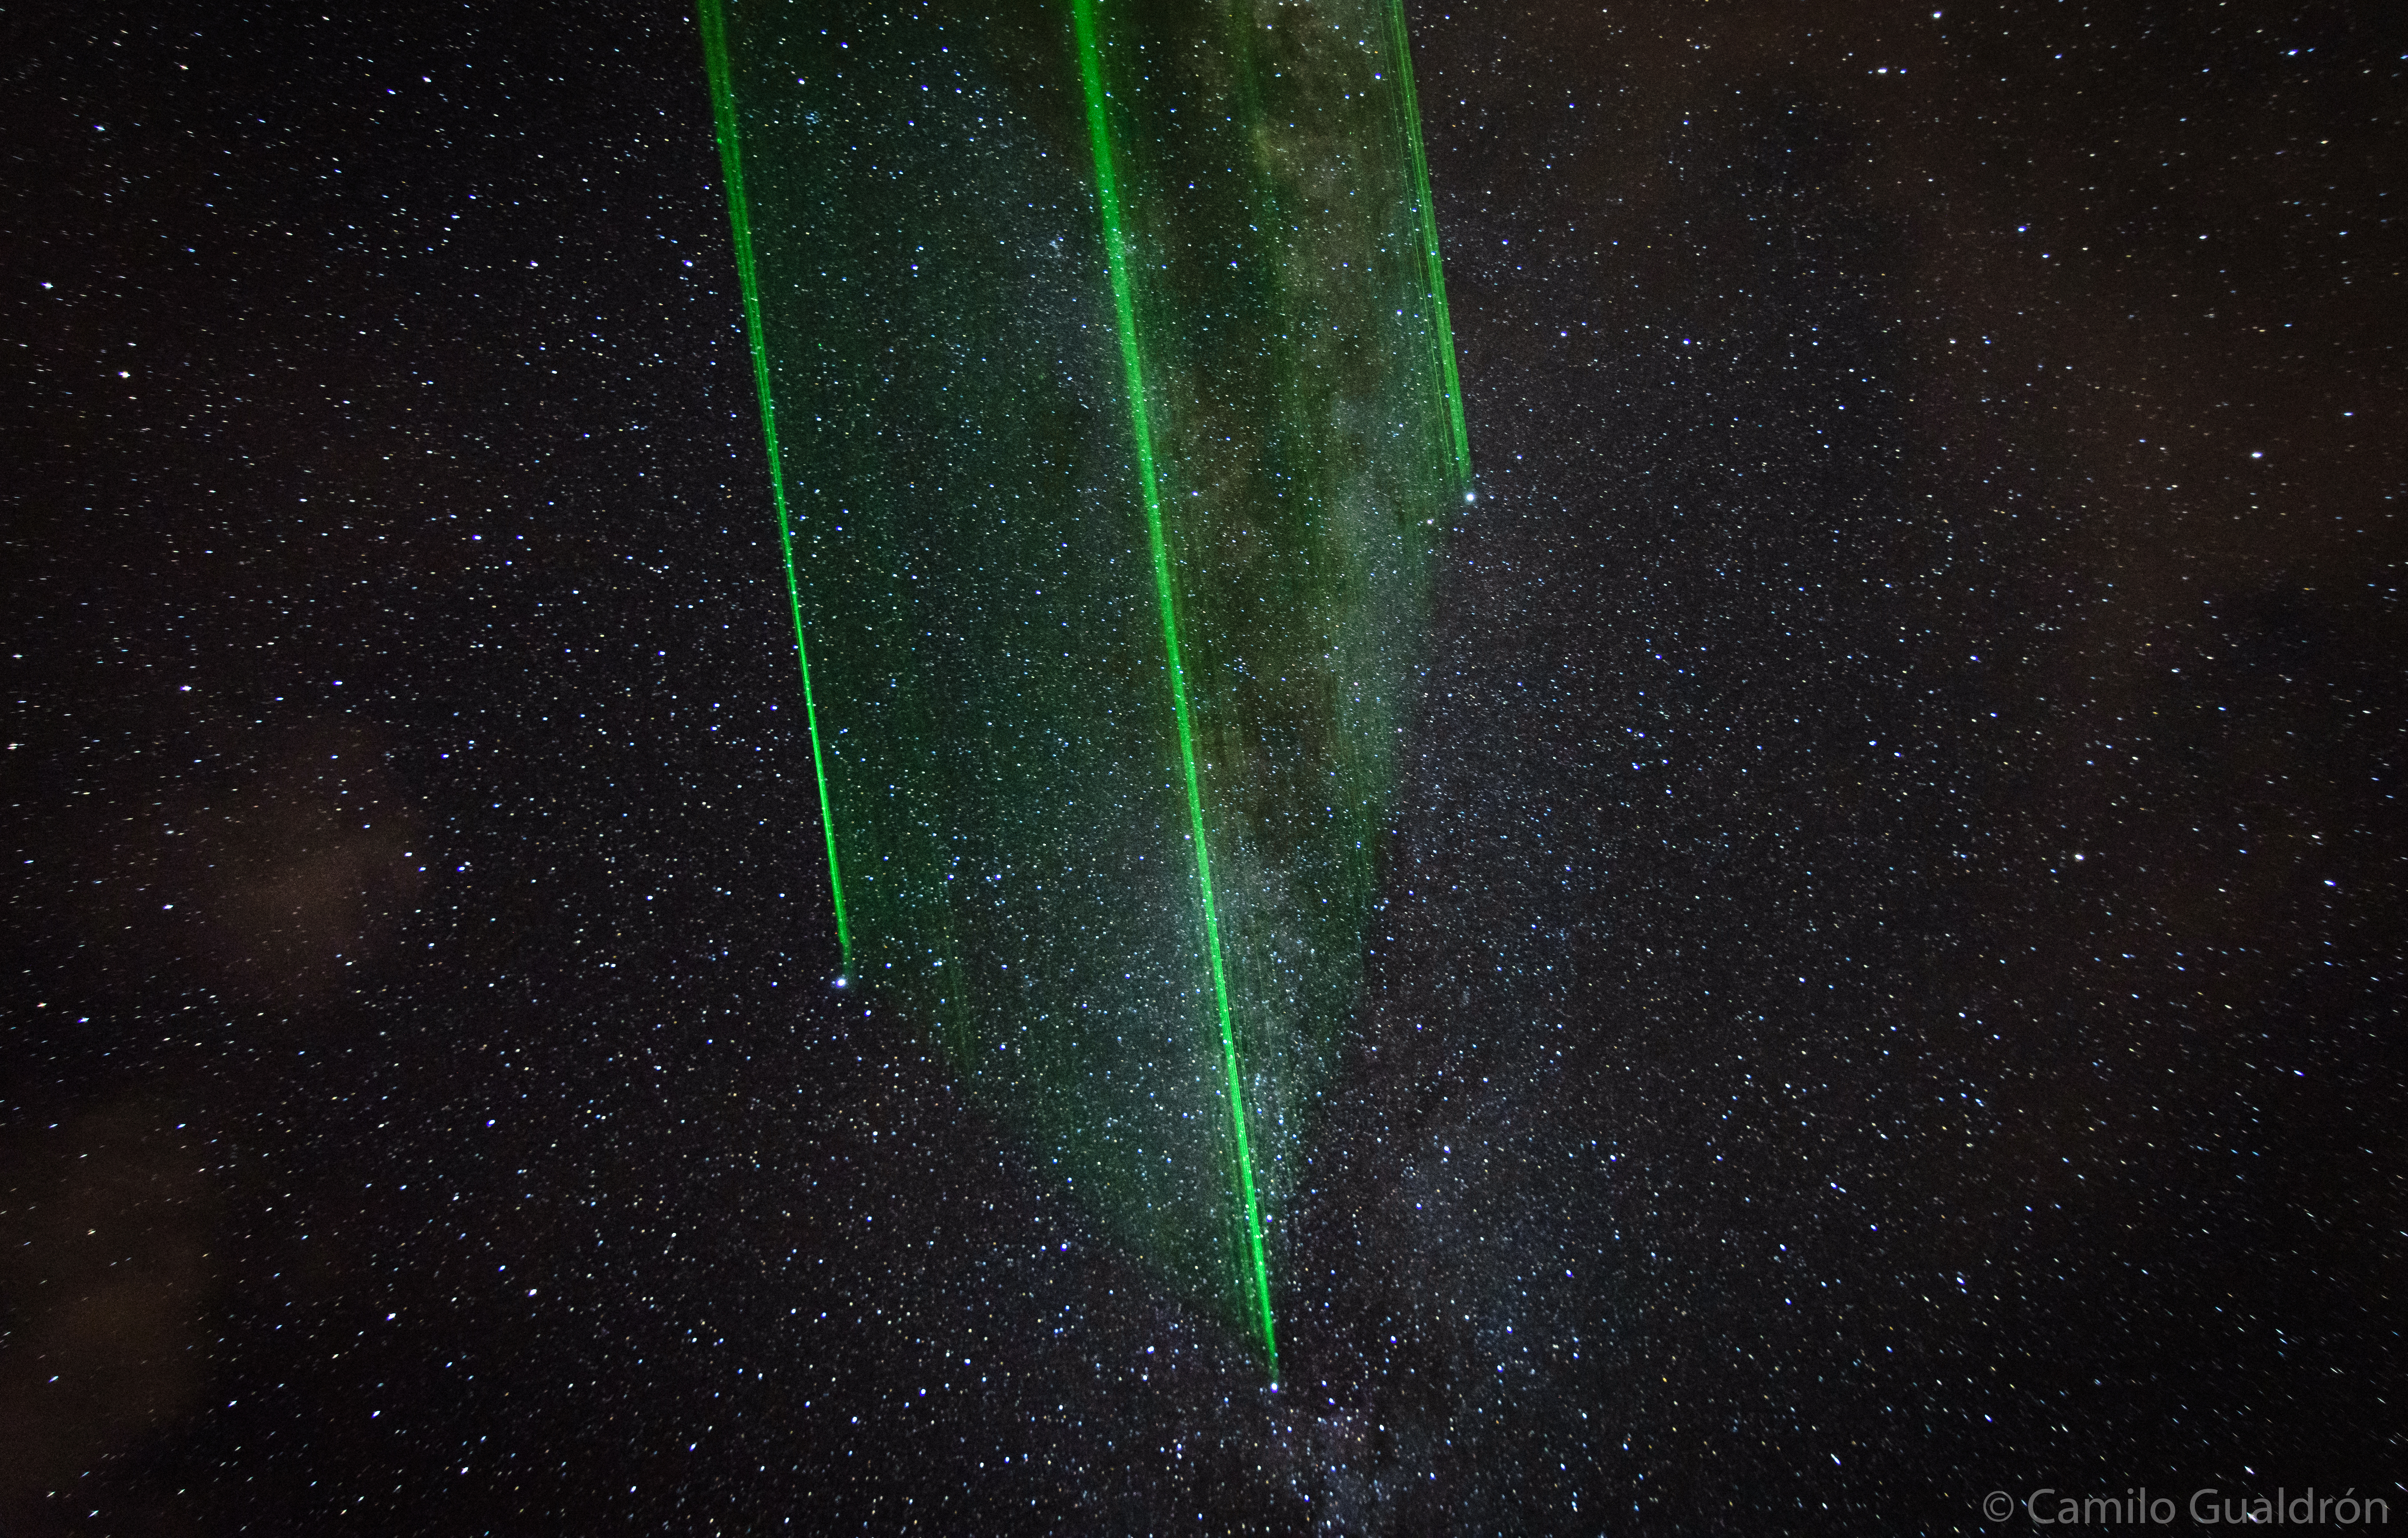
\includegraphics[scale=0.5]{Imagenes/Triangulo_verano}
 \end{figure}
\end{frame}

%%%%%%%%%%%%%%%%%%%%%%%%%%%%%%%%%%%%%%%%%%%%%%%%%%%%%%%%%%%%%%%%%%%%%%%%%%%%%%%%%%%%%%

\begin{frame}{Tales De Mileto}
\begin{columns}
\column{.45\textwidth}
\begin{figure}
 \centering
%\raggedright
 \includegraphics[scale=0.5]{Imagenes/Tales_De_Mileto}
 \end{figure}
 \begin{center}
 \small
 Tales De Mileto
 \end{center}
\column{.45\textwidth}
\begin{itemize}
\item 625 a.C. - 546 a.C.
\item Se puede considerar como el primer gran astrónomo occidental
\item Teorema de Tales
\item Fue el primero en predecir un eclipse
\end{itemize}
\end{columns}
\end{frame}

%%%%%%%%%%%%%%%%%%%%%%%%%%%%%%%%%%%%%%%%%%%%%%%%%%%%%%%%%%%%%%%%%%%%%%%%%%%%%%%%%%%%%%%

\begin{frame}
\begin{figure}
 \centering
%\raggedright
 \includegraphics[scale=0.14]{Imagenes/Eclipse_solar}
 \end{figure}
\end{frame}

%%%%%%%%%%%%%%%%%%%%%%%%%%%%%%%%%%%%%%%%%%%%%%%%%%%%%%%%%%%%%%%%%%%%%%%%%%%%%%%%%%%%%%%%%%%%%%

\begin{frame}{Aristoles} 
\begin{columns}
\column{.45\textwidth}
\begin{figure}
 \centering
%\raggedright
 \includegraphics[scale=0.2]{Imagenes/Aristoteles}
 \end{figure}
 \begin{center}
 \small
 Aristóteles 
 \end{center}
\column{.45\textwidth}
\begin{itemize}
\item 427 a.C. - 347 a.C.
\item Acuño el termino planetas
\item Formula un sistema geocéntrico
\end{itemize}
\end{columns}
\end{frame}

%%%%%%%%%%%%%%%%%%%%%%%%%%%%%%%%%%%%%%%%%%%%%%%%%%%%%%%%%%%%%%%%%%%%%%%%%%%

\begin{frame}
\begin{figure}
 \centering
%\raggedright
 \includegraphics[scale=0.6]{Imagenes/Geocentrico}
 \end{figure}
\end{frame}

%%%%%%%%%%%%%%%%%%%%%%%%%%%%%%%%%%%%%%%%%%%%%%%%%%%%%%%%%%%%%%%%%%%%%%%%%%%%%%

\begin{frame}{Copérnico}
\begin{columns}
\column{.45\textwidth}
\begin{figure}
 \centering
%\raggedright
 \includegraphics[scale=0.6]{Imagenes/Copernico}
 \end{figure}
 \begin{center}
 \small
 Copérnico 
 \end{center}
\column{.45\textwidth}
\begin{itemize}
\item 1473 - 1543 
\item Matemático - Astrónomo - Físico 
\item Sistema heliocéntrico 
\end{itemize}
\end{columns}
\end{frame}

%%%%%%%%%%%%%%%%%%%%%%%%%%%%%%%%%%%%%%%%%%%%%%%%%%%%%%%%%%%%%%%%%%%%%%%%%%%%%%%

\begin{frame}
\begin{figure}
 \centering
%\raggedright
 \includegraphics[scale=0.8]{Imagenes/boveda_celeste_copernico}
 \end{figure}
\end{frame}

%%%%%%%%%%%%%%%%%%%%%%%%%%%%%%%%%%%%%%%%%%%%%%%%%%%%%%%%%%%%%%%%%%%%%%%%%%%%%%%%%%%%
\begin{frame}
\begin{figure}
 \centering
%\raggedright
 \includegraphics[scale=0.7]{Imagenes/Helio_Geo}
 \end{figure}
\end{frame}
%%%%%%%%%%%%%%%%%%%%%%%%%%%%%%%%%%%%%%%%%%%%%%%%%%%%%%%%%%%%%%%%%%%%%%%%%%%%%%%%%%%%

\begin{frame}{Galileo}
\begin{columns}
\column{.45\textwidth}
\begin{figure}
 \centering
%\raggedright
 \includegraphics[scale=2.5]{Imagenes/Galileo}
 \end{figure}
 \begin{center}
 \small
 Galileo  
 \end{center}
\column{.45\textwidth}
\begin{itemize}
 \item 1564 - 1642 
 \item Astrónomo 
 \item Implementó instrumentos ópticos en sus observaciones  
 \item Experimentó con caída libre y péndulos 
 \item Estableció un método científico 
\end{itemize}
\end{columns}
\end{frame}

%%%%%%%%%%%%%%%%%%%%%%%%%%%%%%%%%%%%%%%%%%%%%%%%%%%%%%%%%%%%%%%%%%%%%%%%%%%%%%%%%%%%

\begin{frame}
 \begin{columns}
  \column{.45\textwidth}
  \begin{center}  
  \Huge
   \textbf{Manchas solares}
  \end{center}  
  \column{.45\textwidth}
   \begin{figure}
    \centering
    %\raggedright
    \includegraphics[scale=0.3]{Imagenes/m_s}
  \end{figure}
 \end{columns}
\end{frame}

%%%%%%%%%%%%%%%%%%%%%%%%%%%%%%%%%%%%%%%%%%%%%%%%%%%%%%%%%%%%%%%%%%%%%%%%%%%%%%%%%%%%%

\begin{frame}
 \begin{columns}
  \column{.45\textwidth}
  \begin{center}
  \Huge
  \textbf{Fases de la Luna}
  \end{center}
    \column{.45\textwidth}
   \begin{figure}
    \centering
    %\raggedright
    \includegraphics[scale=0.6]{Imagenes/fases_lunares}
  \end{figure}
 \end{columns}
\end{frame}

%%%%%%%%%%%%%%%%%%%%%%%%%%%%%%%%%%%%%%%%%%%%%%%%%%%%%%%%%%%%%%%%%%%%%%%%%%%%%%%%%%%%


\begin{frame}
 \begin{columns}
  \column{.45\textwidth}
  \begin{center}
  \Huge
  \textbf{Lunas de Júpiter}
  \end{center}
  \column{.45\textwidth}
   \begin{figure}
    \centering
    %\raggedright
    \includegraphics[scale=0.5]{Imagenes/Lunas_jupiter}
  \end{figure}
 \end{columns}
\end{frame}

%%%%%%%%%%%%%%%%%%%%%%%%%%%%%%%%%%%%%%%%%%%%%%%%%%%%%%%%%%%%%%%%%%%%%%%%%%%%%%%%%%%

\begin{frame}
\begin{center}
\Huge
\textbf{\textit{Eppur si muove}}
\end{center}
\end{frame}

%%%%%%%%%%%%%%%%%%%%%%%%%%%%%%%%%%%%%%%%%%%%%%%%%%%%%%%%%%%%%%%%%%%%%%%%%%%%%%%%%%%%%

%%%%%%%%%%%%%%%%%%%%%%%%%%%%%%%%%%%%%%%%%%%%%%%%%%%%%%%%%%%%%%%%%%%%%%%%%%%%%%%%%%%%%
\end{document}